\usepackage{datetime}
\title{A Note on Limits on Incentive Compatibility and Griefing Factors}
\author{
        Vitalik Buterin \\
        Ethereum Foundation
}
\date{\today}
\usepackage{graphicx}

\documentclass[12pt]{article}

\begin{document}
\maketitle
\begin{abstract}
We show a fundamental tradeoff between extortion resistance and griefing resistance in the presence of non-uniquely-attributable faults: if extortion attacks in a consensus mechanism are unprofitable as long as portion $h$ of participants refuses to be extorted, then the mechanism has a griefing factor of at least $\frac{1}{2h} - 1$. We then discuss the notion of variable griefing factors, and propose a methodology for computing penalties for various participants given a particular honest (i.e. unextortable) minority assumption.
\end{abstract}

\section{Introduction}
Consider the general class of mechanisms where there exist an infinite set of infinitesimally small participants, and these participants have three strategies available: \textit{online}, \textit{offline} and \textit{censor}. Censoring participants choose as an argument the victims of the censorship. The mechanism has a partial view of what is going on: it can only see if participants are \textit{present} or \textit{absent}. It determines presence and absence as follows: there exists a set of size $\ge \frac{1}{2}$ of participants that is censoring the same participant set $P$, then any participant $p \in P$ is absent. A participant $p \not \in P$ (or, if no such $P$ exists, any participant $p$) is deemed present if they are online, and absent if they are offline. We deem this a reasonable approximation of consensus games, where being censored and being offline are, from the point of view of a majority chain, indistinguishable. The mechanism imposes some penalty to present validators and some penalty to absent validators (both penalties may depend on the total fraction of validators present).

We explore an "extortion attack", where an attacker (participant set $A$ of size $\ge \frac{1}{2}$) charges an extortion fee $f$, censoring all who do not pay up. Suppose $P_C$ is the mechanism-imposed penalty to a \textit{coalition member} (attacker or someone who pays the extortion fee), and $P_V$ is the prenalty to all others (\textit{victims}). Suppose portion $h$ of participants is "honest" (ie. unextortable). The cost paid by the attacker is $P_C * \frac{1}{2}$. The revenue from extortion is the size of the extorted size $\frac{1}{2} - h$ multiplied by the maximum possible extortion fee, $P_V - P_C$ (the difference between the loss of a victim and the loss of a coalition member; if the extortion fee was higher, it would not be rational to pay up).

\section{Analysis}

For extortion to be unprofitable, we must have:

$-\frac{1}{2} * P_C + (\frac{1}{2} - h) * (P_V - P_C) \le 0$

This can be rewritten:

$-\frac{1}{2} * P_C - (\frac{1}{2} - h) * P_C + (\frac{1}{2} - h) * P_V \le 0$

$(h - 1) * P_C \le (h - \frac{1}{2}) * P_V$

$\frac{P_C}{P_V} \ge \frac{\frac{1}{2} - h}{1 - h}$

Now, without loss of generality suppose $P_V = h - 1$ and $P_C = h - \frac{1}{2}$. We know from the above that the actual values are either these values or these values with two possible deviations: (i) scaling by some constant factor (ignorable because it does not change the griefing ratio) or (ii) setting $P_C$ \textit{higher} than the minimum (this increases the numerator of the below equation and hence makes the griefing factor even higher). Now, consider the scenario where fraction $h$ of participants are the attackers, and they attack by simply going offline. The griefing factor is total victim loss divided by total attacker loss, so it can be computed as:

$\frac{(1 - h) * (\frac{1}{2} - h)}{h * (1 - h)}$

$\frac{\frac{1}{2} - h}{h}$

$\frac{1}{2h} - 1$

If the honest minority assumption used is of size $\frac{1}{3}$, then the griefing factor must be at least $\frac{1}{2}$. If the honest minority assumption is of size $\frac{1}{4}$, then the griefing factor must be at least 1. If the honest minority assumption is of size $\frac{1}{8}$, then the griefing factor must be at least 3.

\section{Hugging the Wall}

One possible reaction to the above is as follows. The proof only shows that, if extortion is unprofitable with an honest minority of size $h$, then the griefing factor \textit{for a griefing attacker of size $h$} is $\frac{1}{2h} - 1$. Having high griefing factors \textit{in the specific case of small attackers} is not that bad, as the consequences are limited in size. So can we come up with a mechanism that "hugs the wall"; where the griefing factor is $\frac{1}{2}$ if the portion of absent participants is $\frac{1}{3}$, the griefing factor is 1 if the portion of absent participants is $\frac{1}{4}$, and so on?

We can show a relation for $P_C(\alpha)$ and $P_V(\alpha)$, where $\alpha$ is the portion of participants absent, that must hold for any hypothetical strategy that does hug the wall in terms of non-exploitability. We know:

$\frac{P_C(\alpha)}{P_V(\alpha)} \ge \frac{\alpha - \frac{1}{2}}{\alpha - 1}$

This is the same formula as one we saw above, but rewritten to make more explicit that $P_C$ and $P_V$ can both depend on $\alpha$. Let us rewrite this in the form of $P_C$, a penalty that everyone pays, and $P_A$, an extra penalty paid by absent participants, so $P_V = P_C + P_A$. We have:

$1 + \frac{P_A(\alpha)}{P_C(\alpha)} \le \frac{\alpha - 1}{\alpha - \frac{1}{2}}$

$1 + \frac{P_A(\alpha)}{P_C(\alpha)} \le 1 - \frac{\frac{1}{2}}{\alpha - \frac{1}{2}}$

$\frac{P_A(\alpha)}{P_C(\alpha)} \le \frac{1}{1 - 2\alpha}$

$P_A(\alpha) * (1 - 2\alpha) \le P_C(\alpha)$

We can achieve optimally low griefing factors if this holds with strict equality. We can also derive an optimal form for $P_C(\alpha)$. We know that we must have $P_C(0) = 0$ (if no participants are absent, no one should be punished, as that is the mechanism's "base case"). We want $P_C(\alpha)$ for $\alpha > 0$ to be positive to penalize censorship. To maximize penalties for any extortion attack where even one participant refuses to be extorted one could consider the formula:

\begin{array}
      $\alpha = 0$: $P(\alpha) = 0$ \\
      $\alpha > 0$: $P(\alpha) = 1$ \\
\end{array}

However, this has the problem that if some portion of participants is \textit{naturally offline} (eg. because people's computers don't always work), then there is no longer any marginal censorship penalty. If we assume no knowledge about what portion of participants is likely to be naturally offline, then the most sensible formula for $P_C(\alpha)$ is that which maintains the same derivative everywhere so as to consistently punish censorship no matter what the quantity or starting conditions. Hence, we have $P_C(\alpha) = k * \alpha$.

From the above formula, we can then derive $P_A = k * \frac{\alpha}{1 - 2\alpha}$. One can check that these rules "hug the wall" perfectly: if an attacker has portion $\alpha$ of participants, and takes them all offline, then the griefing factor is $\frac{1}{2\alpha} - 1$, and an extortion attack in the best case leads to exactly zero revenue (in practice it will be costly because the attacker won't be able to capture literally 100\% of $P_A$ from extortion fees). If we are willing to accept higher griefing factors in exchange for making extortion attacks even more costly, a simple way to do this is to increase $P_C$ relative to $P_A$.

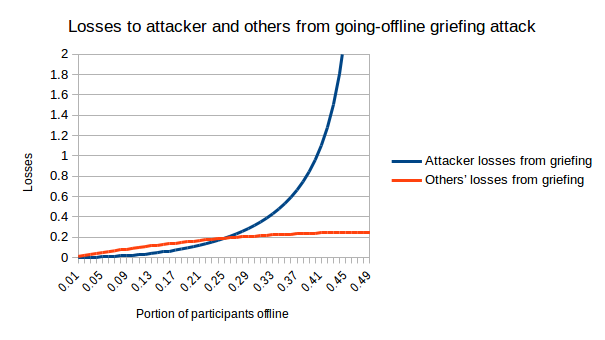
\includegraphics{chart1.png}
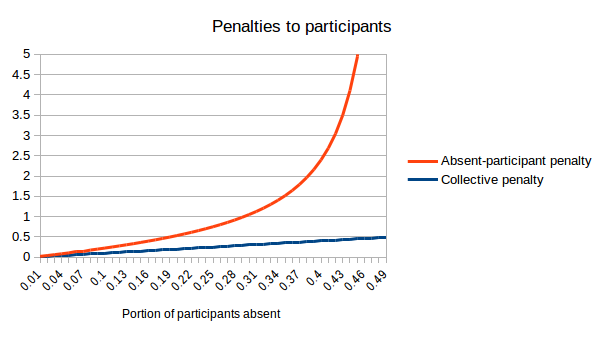
\includegraphics{chart2.png}
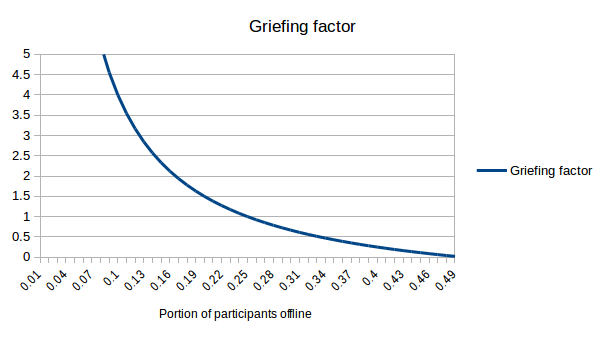
\includegraphics{chart3.png}

The formulas as given are likely not a good idea, as a griefing factor below $\frac{1}{2}$ for participants going offline implies a griefing factor greater than 2 for large-scale censorship. Hence, adding a "floor" at $\frac{1}{2}$ may be optimal. Additionally, if we are willing to accept an "honest majority" assumption of some $h$; that is, assume that fraction $h$ will never listen to an extortionist, then we can cap griefing factors even for small-scale griefing attacks. This can be accomplished by clamping $P_A$:

$P_A(\alpha) = clamp(h, \frac{\alpha}{1 - 2\alpha}, 1)$

\section{Conclusions}\label{conclusions}
An honest minority model is a necessary part of a consensus mechanism's ability to resist extortion. The smaller the assumes honest minority, the higher the griefing factors that the protocol exposes itself to. However, if we are comfortable with accepting higher griefing factors for smaller attackers, then we can create penalty formulas that achieve closer-to-optimal results across a wide range of attacker sizes, although it becomes necessary for the penalty incurred by an absent participant for being absent to itself depend on the number of other absent participants.

\bibliographystyle{abbrv}
\bibliography{main}

\end{document}
